% Provenance (never printed): cycle 4 SVT, "La planete Terre, l'environnement
% et l'action humaine": natural risks, hazard and vulnerability, prevention
% and protection; see sources/book1/PROVENANCE.md. Book 1, grade 9, chapter 2.
% Vocabulary guard: owns risk, vulnerability, prevention, hazard map.
% Natural hazard and natural disaster, the warning colours and the safety
% rules are g5's (natural-hazards); the warning signs of an eruption and the
% Pinatubo story are g7's (volcanoes); seismometer, tsunami and "scientists
% cannot predict earthquakes" are g7's (earthquakes); flood and floodplain
% are g5's (water-shapes-the-land); weather forecast is g8's. Lahars are
% called mudflows (as in g7). "Normal fault" is Book 2's: here "a fault".
\chapter{Vivre avec les risques naturels}\label{ch:g9:natural-risks}

Tard dans la soirée du 13~novembre 1985, la plupart des habitants
d'Armero, une ville de Colombie, étaient couchés. Un orage cachait le
\omterm{def:g4:volcanoes-earthquakes-first-look:volcano}{volcan} enneigé du Nevado del Ruiz, à \qty{45}{km} de là, et personne en
ville ne le vit entrer en \omterm{def:g4:volcanoes-earthquakes-first-look:eruption}{éruption}. Les \omterm{def:g3:stones-pebbles-sand:rock}{roches} brûlantes firent fondre une
partie de sa glace, et l'eau, mêlée de cendres et de \omterm{def:g3:stones-pebbles-sand:rock}{roches}, dévala les
\omterm{def:g1:landscapes-around-us:landform}{vallées} en coulées de boue. Environ deux heures plus tard, les coulées de
boue sortirent de la \omterm{def:g1:landscapes-around-us:landform}{vallée} du río Lagunillas, droit sur la ville~:
quelque \num{23000} personnes, la plus grande partie de la ville, furent
tuées. Deux heures, c'était assez pour gagner à pied des terrains plus
élevés. Les habitants d'Armero ne furent pas prévenus.
% ledger: usgs:armero

\begin{omfigure}
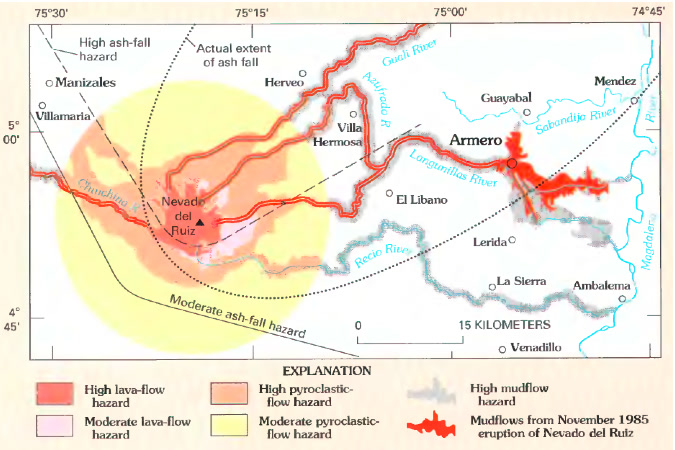
\includegraphics[width=0.86\linewidth]{images/book1/g9-ruiz-hazard-map.jpg}

{\small La \omterm{def:g9:natural-risks:hazard-map}{carte des aléas} du Nevado del Ruiz. Une première version,
établie par des géologues colombiens, circulait un mois avant l'\omterm{def:g4:volcanoes-earthquakes-first-look:eruption}{éruption}
et montrait déjà le danger de coulées de boue dans la \omterm{def:g1:landscapes-around-us:landform}{vallée} d'Armero.
Cette version, redessinée après la catastrophe, ajoute en rouge vif les
coulées de boue réellement survenues en novembre 1985 (le cercle ombré
autour du \omterm{def:g4:volcanoes-earthquakes-first-look:volcano}{volcan} a un rayon d'environ \qty{20}{km}). D'après T.~L.~Wright et
T.~C.~Pierson, USGS Circular 1073, 1992 (domaine public, via Wikimedia
Commons).}
% ledger: usgs:ruiz-map, commons:ruiz-map
\label{fig:g9:natural-risks:ruiz}
\end{omfigure}

Six ans plus tard, au mont Pinatubo, aux Philippines, le \omterm{def:g4:volcanoes-earthquakes-first-look:volcano}{volcan} était
surveillé, l'alerte fut donnée à temps et la population partit
(\cref{ch:g7:volcanoes}). Les deux étaient des \omterm{def:g4:volcanoes-earthquakes-first-look:volcano}{volcans} explosifs, avec des
habitants vivant sur le trajet de leurs coulées de boue. Ce qui différait,
c'était ce que les gens savaient, et ce qu'ils en firent. Ce chapitre
porte sur cette différence.
% ledger: usgs:armero (Pinatubo 1991 averted a disaster like Armero), usgs:pinatubo-1991

\begin{recall}
Un \emph{\omterm{def:g5:natural-hazards:hazard}{aléa naturel}} est un phénomène naturel qui peut nuire aux
êtres humains~; il devient une \emph{\omterm{def:g5:natural-hazards:disaster}{catastrophe naturelle}} quand il
frappe là où des gens vivent et cause de grands dommages
(\cref{ch:g5:natural-hazards}). Une \omterm{def:g1:landscapes-around-us:water}{rivière} qui déborde recouvre sa \omterm{def:g5:water-shapes-the-land:flood}{plaine
d'inondation} (\cref{ch:g5:water-shapes-the-land}). Un \omterm{def:g4:volcanoes-earthquakes-first-look:volcano}{volcan} donne souvent
des signes avant-coureurs avant une grande \omterm{def:g4:volcanoes-earthquakes-first-look:eruption}{éruption}~: petits \omterm{def:g4:volcanoes-earthquakes-first-look:earthquake}{séismes},
gonflement des pentes, gaz (\cref{ch:g7:volcanoes}). Les scientifiques ne
savent pas prévoir les \omterm{def:g4:volcanoes-earthquakes-first-look:earthquake}{séismes}~; les \omterm{def:g7:earthquakes:seismometer}{sismomètres} les enregistrent, et un
\omterm{def:g4:volcanoes-earthquakes-first-look:earthquake}{séisme} sous la \omterm{def:g2:water-on-earth:ocean}{mer} peut déclencher un \omterm{def:g7:earthquakes:tsunami}{tsunami} (\cref{ch:g7:earthquakes}).
Une \omterm{def:g8:fronts-and-weather-maps:forecast}{prévision météorologique} dit quel temps il fera dans les jours qui
viennent (\cref{ch:g8:fronts-and-weather-maps}).
\end{recall}

\section{Aléa, vulnérabilité et risque}

Le même \omterm{def:g4:volcanoes-earthquakes-first-look:earthquake}{séisme} ne fait pas les mêmes dégâts partout. Sous un \omterm{def:g5:weather-and-climate:desert}{désert} vide,
il ne fait de mal à personne. Sous une ville aux bâtiments solides dont
les habitants savent quoi faire, il secoue, effraie et brise des vitres.
Sous une ville de maisons lourdes et mal construites, il peut les faire
s'écrouler sur leurs occupants. L'aléa est le même~; ce qui change, c'est
la facilité avec laquelle le lieu peut subir des dommages.

\begin{definition}[Vulnérabilité]\label{def:g9:natural-risks:vulnerability}
La \emph{vulnérabilité}\index{vulnerabilite@vulnérabilité} d'un lieu est la facilité avec
laquelle ses habitants, ses bâtiments et ce dont ils ont besoin peuvent
subir des dommages causés par un \omterm{def:g5:natural-hazards:hazard}{aléa naturel}. Des habitations dans une
\omterm{def:g5:water-shapes-the-land:flood}{plaine d'inondation}, des bâtiments fragiles, aucune alerte et aucun plan
rendent un lieu vulnérable.
\end{definition}

\begin{definition}[Risque]\label{def:g9:natural-risks:risk}
Le \emph{risque}\index{risque} auquel un lieu est exposé face à un \omterm{def:g5:natural-hazards:hazard}{aléa naturel} est
le danger de dommages pour ses habitants et leurs biens. Il dépend à la
fois de l'aléa, de sa force et de sa fréquence, et de la \omterm{def:g9:natural-risks:vulnerability}{vulnérabilité} du
lieu~: là où il n'y a pas d'aléa, ou rien qui puisse subir de dommages, il
n'y a pas de risque.
\end{definition}

\begin{omfigure}
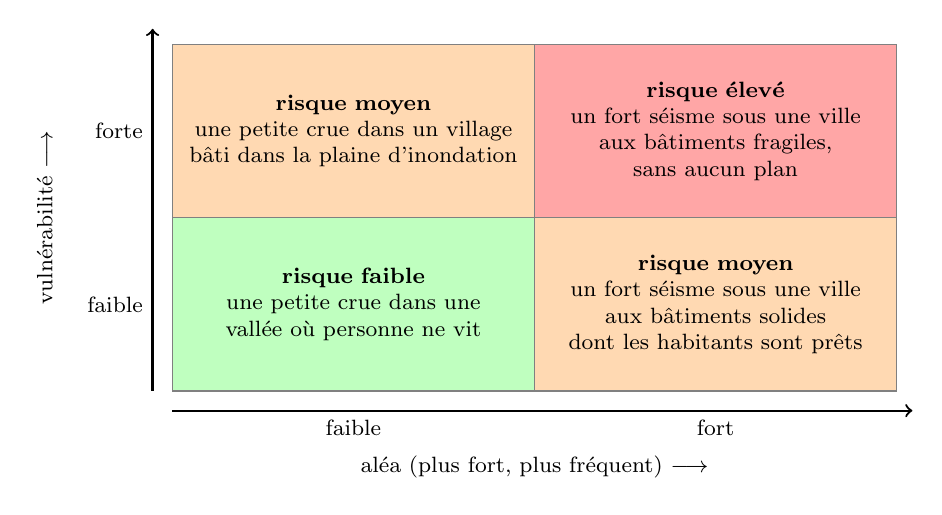
\begin{tikzpicture}[x=1cm, y=1cm, font=\footnotesize,
    cell/.style={minimum width=4.6cm, minimum height=2.2cm, align=center, draw=black!50, text width=4.2cm}]
  \node[cell, fill=green!25] at (2.3,1.1) {\textbf{risque faible}\\ une petite crue dans une\\ vallée où personne ne vit};
  \node[cell, fill=orange!30] at (6.9,1.1) {\textbf{risque moyen}\\ un fort séisme sous une ville\\ aux bâtiments solides\\ dont les habitants sont prêts};
  \node[cell, fill=orange!30] at (2.3,3.3) {\textbf{risque moyen}\\ une petite crue dans un village\\ bâti dans la plaine d'inondation};
  \node[cell, fill=red!35] at (6.9,3.3) {\textbf{risque élevé}\\ un fort séisme sous une ville\\ aux bâtiments fragiles,\\ sans aucun plan};
  \draw[->, thick] (0,-0.25) -- (9.4,-0.25);
  \draw[->, thick] (-0.25,0) -- (-0.25,4.6);
  \node[anchor=north] at (4.6,-0.7) {aléa (plus fort, plus fréquent) $\longrightarrow$};
  \node[rotate=90, anchor=south] at (-1.4,2.2) {vulnérabilité $\longrightarrow$};
  \node[below] at (2.3,-0.25) {faible};
  \node[below] at (6.9,-0.25) {fort};
  \node[left] at (-0.25,1.1) {faible};
  \node[left] at (-0.25,3.3) {forte};
\end{tikzpicture}

{\small La grille du \omterm{def:g9:natural-risks:risk}{risque} (un croquis). Le \omterm{def:g9:natural-risks:risk}{risque} augmente avec l'aléa
et avec la \omterm{def:g9:natural-risks:vulnerability}{vulnérabilité}. Déplacer une ville est rarement possible, et on
ne peut pas éteindre un aléa~; mais on peut réduire la \omterm{def:g9:natural-risks:vulnerability}{vulnérabilité} de
la ville, ce qui la fait descendre dans la grille.}
\label{fig:g9:natural-risks:grid}
\end{omfigure}

Armero était un lieu d'aléa fort~: un \omterm{def:g4:volcanoes-earthquakes-first-look:volcano}{volcan} enneigé qui s'était réveillé
un an plus tôt, et une ville bâtie sur les \omterm{def:g5:water-shapes-the-land:deposition}{dépôts} d'anciennes coulées de
boue, au débouché d'une \omterm{def:g1:landscapes-around-us:landform}{vallée} qui en avait déjà charrié. La ville était
aussi très vulnérable~: les scientifiques manquaient d'instruments et de
soutien, les informations transmises aux autorités étaient souvent
vagues, et il n'existait ni plan d'évacuation ni moyen rapide d'alerter la
ville.
% ledger: usgs:armero

\section{Prévoir et prévenir}

Certains aléas se voient venir. Une \omterm{def:g5:natural-hazards:storm}{tempête} est prévue plusieurs jours à
l'avance (\cref{ch:g8:fronts-and-weather-maps})~; une \omterm{def:g5:water-shapes-the-land:flood}{crue} après de
fortes \omterm{def:g4:clouds-rain-snow:precipitation}{pluies}, quelques heures à quelques jours à l'avance~; une grande
\omterm{def:g4:volcanoes-earthquakes-first-look:eruption}{éruption} s'annonce souvent quelques jours à quelques semaines à l'avance,
mais pas toujours. Un \omterm{def:g7:earthquakes:tsunami}{tsunami} traverse un \omterm{def:g2:water-on-earth:ocean}{océan} en quelques heures, si
bien qu'une alerte peut atteindre les \omterm{def:g1:landscapes-around-us:water}{côtes} lointaines avant lui. Les
\omterm{def:g4:volcanoes-earthquakes-first-look:earthquake}{séismes}, en revanche, ne peuvent pas être prévus~: les scientifiques
peuvent dire quelles \omterm{def:g7:earthquakes:fault}{failles} rompront de nouveau un jour, jamais quel
jour.
% ledger: nws:tsunami-speed, usgs:eq-basics, usgs:pinatubo-1991

Une prévision, aussi bonne soit-elle, n'est utile que si l'on agit avant
que l'aléa ne frappe. L'essentiel de ce travail se fait bien avant toute
alerte.

\begin{definition}[Prévention]\label{def:g9:natural-risks:prevention}
La \emph{prévention}\index{prevention@prévention} est tout ce que l'on fait avant qu'un \omterm{def:g5:natural-hazards:hazard}{aléa
naturel} ne frappe pour réduire le \omterm{def:g9:natural-risks:risk}{risque}~: savoir où l'aléa peut frapper,
construire à des endroits sûrs et de manière sûre, surveiller l'aléa,
alerter la population et la préparer.
\end{definition}

La \omterm{def:g9:natural-risks:prevention}{prévention} agit des deux côtés de la grille du \omterm{def:g9:natural-risks:risk}{risque}. Surveiller un
\omterm{def:g4:volcanoes-earthquakes-first-look:volcano}{volcan} ou une \omterm{def:g1:landscapes-around-us:water}{rivière} ne les rend pas moins dangereux, mais cela donne le
temps d'agir. Construire loin de la \omterm{def:g5:water-shapes-the-land:flood}{plaine d'inondation}, bâtir des maisons
solides, prévoir les itinéraires vers les hauteurs et s'y entraîner~:
tout cela réduit la \omterm{def:g9:natural-risks:vulnerability}{vulnérabilité}.

\begin{omfigure}
\begin{minipage}[c]{0.44\linewidth}\centering
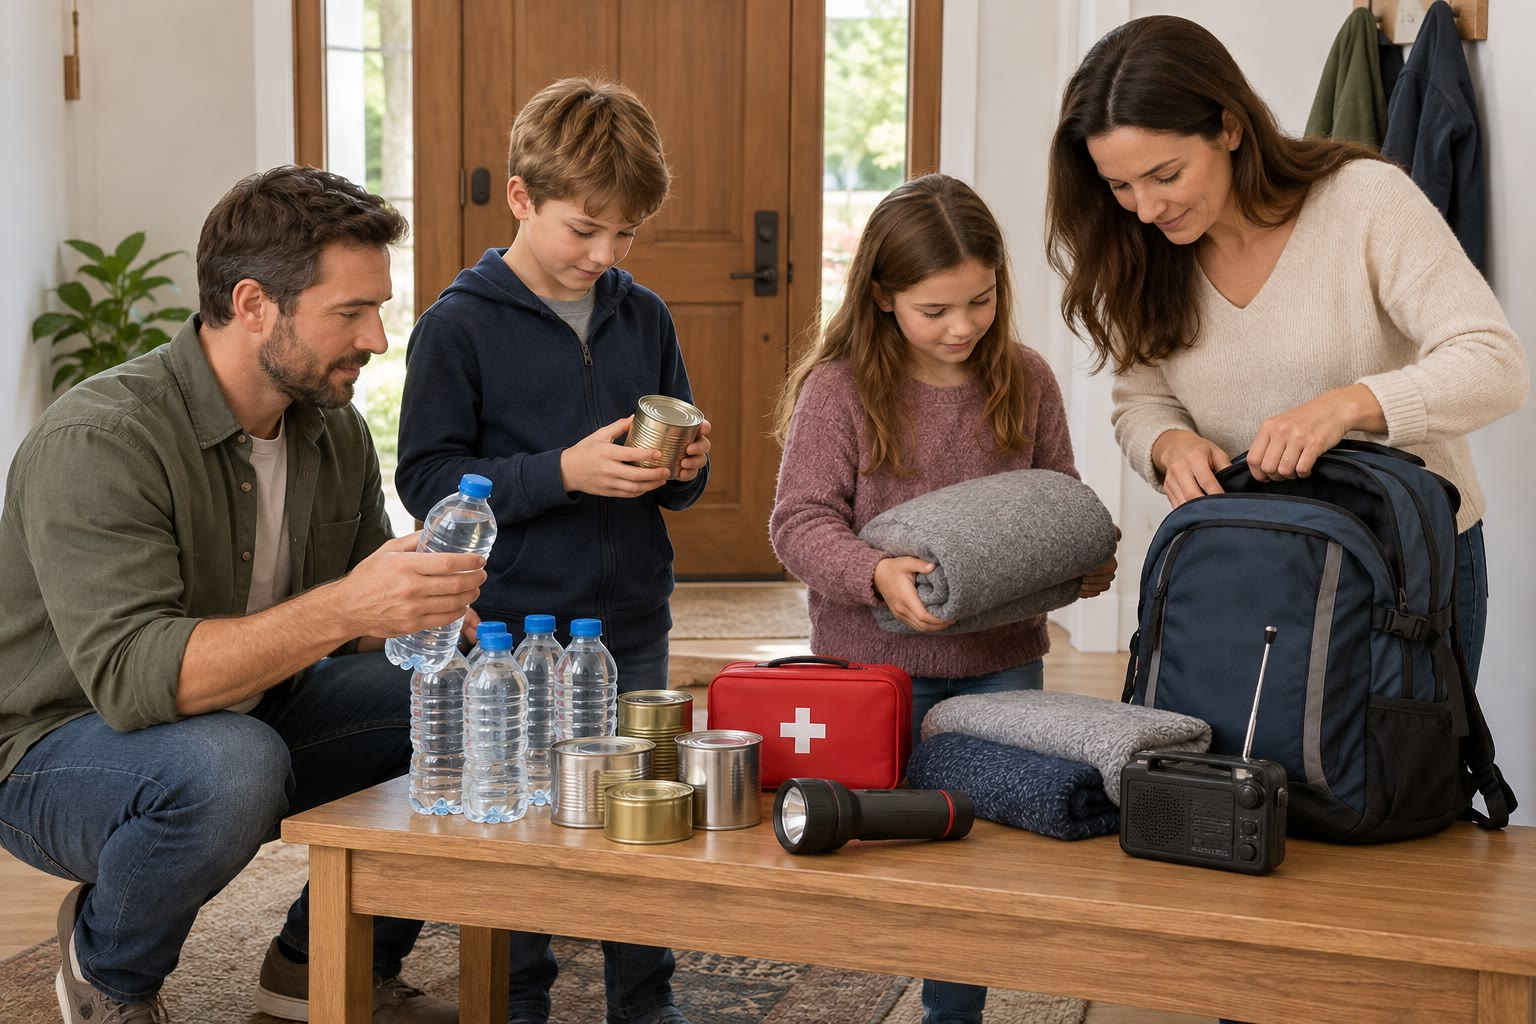
\includegraphics[width=\linewidth]{images/book1/ai/g9-emergency-kit.jpg}
\end{minipage}\hfill
\begin{minipage}[c]{0.52\linewidth}\raggedright
{\small Être prêt~: une famille vérifie son kit d'urgence, rangé près de
la porte, prêt à emporter s'il faut partir vite~: de l'eau et de la
nourriture qui se conservent plusieurs jours, une lampe de poche, une
radio qui fonctionne sans le secteur, des piles de rechange, une trousse
de premiers secours et des couvertures chaudes (illustration générée par
IA d'une scène générique).}
\end{minipage}
% ledger: ready:kit
\label{fig:g9:natural-risks:kit}
\end{omfigure}

\section{Surveiller les volcans et les failles}

Un observatoire volcanologique surveille les signes avant-coureurs vus au
\cref{ch:g7:volcanoes} avec des instruments qui fonctionnent jour et nuit
et transmettent leurs mesures à l'observatoire.
% ledger: usgs:hvo-toolkit

\begin{omfigure}
\begin{tikzpicture}[x=1cm, y=1cm, font=\footnotesize, >={Stealth[length=2mm]}]
  % ground and cone
  \fill[black!13] (0,0) -- (0,1.0) -- (3.0,1.2) -- (5.4,3.6) -- (6.4,3.6) -- (8.8,1.2) -- (12,1.0) -- (12,0) -- cycle;
  \draw[black!60] (0,1.0) -- (3.0,1.2) -- (5.4,3.6) -- (6.4,3.6) -- (8.8,1.2) -- (12,1.0);
  % magma chamber and conduit
  \fill[omWarm!70] (5.9,0.6) ellipse (1.5 and 0.38);
  \fill[omWarm!70] (5.75,0.9) rectangle (6.05,3.6);
  \node[white, font=\scriptsize\bfseries] at (5.9,0.58) {magma};
  % gas plume, drifting west
  \fill[black!10] (5.8,3.95) circle (0.3) (5.35,4.35) circle (0.4) (4.75,4.75) circle (0.45);
  % swollen east flank, dashed
  \draw[dashed, omWarm, line width=0.8pt] (6.45,3.7) .. controls (7.5,3.55) and (8.6,2.6) .. (8.85,1.25);
  \draw[->, omWarm] (7.3,2.75) -- (7.7,3.15);
  \node[anchor=west, align=left, text=omWarm!80!black] at (8.2,3.75) {le magma qui monte\\ fait gonfler la pente};
  % tiltmeter on the east flank
  \fill[black] (7.75,2.12) rectangle (8.05,2.24);
  \draw[black!70] (8.1,2.2) -- (8.5,2.45);
  \node[anchor=west, align=left] at (8.5,2.55) {inclinomètre~: la pente\\ s'incline en gonflant};
  % GPS receiver on the west flank, and its satellite
  \draw[black, line width=0.6pt] (4.4,2.6) -- (4.4,2.95);
  \fill[black] (4.25,2.95) rectangle (4.55,3.05);
  \draw[black] (4.4,3.05) circle (0.1);
  \draw[black, fill=white] (1.7,4.85) rectangle (2.0,5.05);
  \draw[black] (1.4,4.95) -- (2.3,4.95);
  \node[anchor=east] at (1.35,4.95) {satellite};
  \draw[black!50, dashed] (4.3,3.15) -- (2.05,4.8);
  \draw[black!70] (3.05,2.65) -- (4.2,2.85);
  \node[anchor=east, align=right] at (3.0,2.6) {récepteur GPS~: le\\ sol bouge de\\ quelques millimètres};
  % gas instrument on the crater rim
  \fill[black] (6.45,3.6) rectangle (6.75,3.75);
  \draw[black!70] (6.8,3.75) -- (7.1,4.45);
  \node[anchor=west, align=left] at (7.1,4.6) {analyseur de gaz~: les gaz\\ qui s'échappent du cratère};
  % seismometer (in the ground)
  \fill[black] (2.1,0.95) rectangle (2.4,1.1);
  \node[anchor=north, align=center] at (1.6,0.85) {sismomètre~:\\ petits séismes};
  % camera, east, looking at the summit
  \fill[black] (10.7,1.12) rectangle (11.0,1.32);
  \fill[black] (10.7,1.17) -- (10.55,1.12) -- (10.55,1.32) -- (10.7,1.27) -- cycle;
  \node[anchor=north, align=center] at (10.8,0.85) {caméra~:\\ surveille le sommet};
\end{tikzpicture}

{\small Surveiller un \omterm{def:g4:volcanoes-earthquakes-first-look:volcano}{volcan} (un croquis, sans souci d'échelle). Les
\omterm{def:g7:earthquakes:seismometer}{sismomètres} comptent les petits \omterm{def:g4:volcanoes-earthquakes-first-look:earthquake}{séismes}~; les inclinomètres et les
récepteurs GPS, fixés à la \omterm{def:g3:stones-pebbles-sand:rock}{roche}, mesurent comment le sol s'incline et se
déplace quand le \omterm{def:g7:volcanoes:magma}{magma} s'accumule en profondeur~; d'autres instruments
mesurent les gaz qui s'échappent~; des caméras surveillent le sommet. Des
\omterm{def:g4:clouds-rain-snow:rain-gauge}{pluviomètres} aident à distinguer les signaux du \omterm{def:g4:volcanoes-earthquakes-first-look:volcano}{volcan} des effets de
fortes \omterm{def:g4:clouds-rain-snow:precipitation}{pluies}.}
% ledger: usgs:hvo-toolkit
\label{fig:g9:natural-risks:monitoring}
\end{omfigure}

Aucun de ces signes ne donne le jour et l'heure d'une \omterm{def:g4:volcanoes-earthquakes-first-look:eruption}{éruption}. Les
scientifiques les lisent ensemble, comme un médecin lit plusieurs mesures
d'un patient, et disent comment le danger évolue~; les autorités décident
quand fermer une zone et quand évacuer la population. Au Pinatubo, cette
chaîne a fonctionné. Au Nevado del Ruiz, le \omterm{def:g4:volcanoes-earthquakes-first-look:volcano}{volcan} donnait des signes
depuis un an, avec des essaims de \omterm{def:g4:volcanoes-earthquakes-first-look:earthquake}{séismes}, mais les instruments étaient
peu nombreux, et la chaîne qui allait des scientifiques aux habitants
d'Armero était rompue.
% ledger: usgs:armero, usgs:hvo-toolkit, usgs:pinatubo-1991

Les \omterm{def:g7:earthquakes:fault}{failles} sont surveillées de la même manière, par des réseaux de
\omterm{def:g7:earthquakes:seismometer}{sismomètres} et de stations GPS qui mesurent, millimètre par millimètre,
comment les deux côtés d'une \omterm{def:g7:earthquakes:fault}{faille} se déplacent lentement. On sait ainsi
quelles \omterm{def:g7:earthquakes:fault}{failles} accumulent la tension du prochain grand \omterm{def:g4:volcanoes-earthquakes-first-look:earthquake}{séisme}, mais pas
quand il viendra. Face aux \omterm{def:g4:volcanoes-earthquakes-first-look:earthquake}{séismes}, la \omterm{def:g9:natural-risks:prevention}{prévention} est la principale
défense.
% ledger: usgs:gps, usgs:eq-basics

\section{Cartes des aléas et zones inondables}

La première étape de la \omterm{def:g9:natural-risks:prevention}{prévention} est de savoir où un aléa peut frapper.

\begin{definition}[Carte des aléas]\label{def:g9:natural-risks:hazard-map}
Une \emph{carte des aléas}\index{carte des aleas@carte des aléas} montre les endroits qu'un \omterm{def:g5:natural-hazards:hazard}{aléa
naturel} peut atteindre, souvent avec plusieurs niveaux de danger. Elle est
établie à partir de ce que l'aléa a fait dans le passé et de la forme du
terrain.
\end{definition}

La \omterm{def:g2:drawing-to-map:map}{carte} du Nevado del Ruiz, au début de ce chapitre, est une \omterm{def:g9:natural-risks:hazard-map}{carte des
aléas}~: les coulées de boue du passé avaient suivi les \omterm{def:g1:landscapes-around-us:landform}{vallées}, et les
suivantes les suivraient aussi. Les \omterm{def:g2:drawing-to-map:map}{cartes} des zones inondables reposent
sur la même idée. L'eau s'étale sur les terrains bas et plats qui bordent
une \omterm{def:g1:landscapes-around-us:water}{rivière}~: plus la \omterm{def:g5:water-shapes-the-land:flood}{crue} est haute, plus la bande de terrain qu'elle
recouvre est large. Une \omterm{def:g2:drawing-to-map:map}{carte} des zones inondables trace la limite de
l'eau pour une \omterm{def:g5:water-shapes-the-land:flood}{crue} choisie, souvent la \omterm{def:g5:water-shapes-the-land:flood}{crue} qui a une chance sur 100
d'être atteinte ou dépassée chaque année. On l'appelle la \emph{\omterm{def:g5:water-shapes-the-land:flood}{crue}
centennale}, mais ce n'est pas une \omterm{def:g5:water-shapes-the-land:flood}{crue} qui vient une fois par siècle~:
elle peut survenir deux années de suite.
% ledger: fema:flood-zones

\begin{omfigure}
\begin{tikzpicture}
\begin{axis}[axis equal image, xmin=3.5, xmax=7, ymin=2.7, ymax=5.5, width=11.5cm,
  enlargelimits=false, tick label style={font=\scriptsize}, xlabel={est (km)},
  ylabel={nord (km)}, label style={font=\small}, xtick={3.5,4,...,7}, ytick={3,3.5,...,5.5},
  clip mode=individual]
\addplot[contour] table {figdata/out/grade-9-flood_zone-contours.dat};
\addplot[index contour] table {figdata/out/grade-9-flood_zone-index.dat};
\addplot[fill=omSea, draw=blue!40, line width=0.3pt] table {figdata/out/grade-9-flood_zone-zone10.dat} -- cycle;
\addplot[fill=blue!25, draw=blue!50, line width=0.3pt] table {figdata/out/grade-9-flood_zone-zone.dat} -- cycle;
\addplot[fill=blue!50, draw=none] table {figdata/out/grade-9-flood_zone-zone2.dat} -- cycle;
\addplot[only marks, mark=none, point meta=explicit symbolic, nodes near coords,
  nodes near coords align={center}, nodes near coords style={font=\tiny, fill=white, inner sep=0.6pt, text=omContour}]
  table[meta=z] {figdata/out/grade-9-flood_zone-index-lab.dat};
\addplot[river] table {figdata/out/grade-9-flood_zone-river.dat};
\end{axis}
\end{tikzpicture}

\smallskip
\begin{tikzpicture}[font=\footnotesize]
  \node[anchor=east] at (0,0.125) {crue au-dessus de la rivière~:};
  \fill[blue!50] (0.2,0) rectangle (0.7,0.25); \node[anchor=west] at (0.8,0.125) {\qty{2}{m}};
  \fill[blue!25, draw=blue!50, line width=0.3pt] (1.9,0) rectangle (2.4,0.25); \node[anchor=west] at (2.5,0.125) {\qty{5}{m}};
  \fill[omSea, draw=blue!40, line width=0.3pt] (3.6,0) rectangle (4.1,0.25); \node[anchor=west] at (4.2,0.125) {\qty{10}{m}};
\end{tikzpicture}

{\small La \omterm{def:g5:water-shapes-the-land:flood}{plaine d'inondation} de la \omterm{def:g1:landscapes-around-us:water}{rivière} des collines de Varden, qui
coule vers l'est. Chaque teinte correspond au terrain qu'une \omterm{def:g5:water-shapes-the-land:flood}{crue}
recouvrirait si elle montait à 2, 5 ou \qty{10}{m} au-dessus du niveau
normal de la \omterm{def:g1:landscapes-around-us:water}{rivière}~: chaque zone contient les plus petites. Les zones
restent étroites parce que les versants de la \omterm{def:g1:landscapes-around-us:landform}{vallée} s'élèvent vite
au-dessus de son fond plat. Les lignes fines relient des points de même
\omterm{def:g4:world-physical-map:altitude}{altitude}, tous les \qty{10}{m}, avec une valeur tous les \qty{50}{m}~; ces
\omterm{def:g2:drawing-to-map:map}{cartes} sont le sujet du \cref{ch:g9:maps-of-the-earth}.}
% ledger: (invented region: figdata/grade-9/flood_zone.py, parts zone2, zone, zone10)
\label{fig:g9:natural-risks:flood-zones}
\end{omfigure}

\begin{method}[Lire une carte des zones inondables]
\begin{enumerate}
  \item Repère à quelle \omterm{def:g5:water-shapes-the-land:flood}{crue} correspond la zone~: à quelle hauteur
        au-dessus de la \omterm{def:g1:landscapes-around-us:water}{rivière}, ou à quelle fréquence elle peut survenir.
  \item Situe le lieu sur la \omterm{def:g2:drawing-to-map:map}{carte}, avec l'\omterm{def:g2:drawing-to-map:scale}{échelle} graphique ou le
        quadrillage.
  \item Si le lieu se trouve dans la zone ombrée, cette \omterm{def:g5:water-shapes-the-land:flood}{crue}
        l'atteindrait~; s'il se trouve en dehors, il resterait au sec lors
        de cette \omterm{def:g5:water-shapes-the-land:flood}{crue}, mais pas lors de toutes les \omterm{def:g5:water-shapes-the-land:flood}{crues}.
  \item Pour comparer des lieux, utilise leur hauteur au-dessus de la
        \omterm{def:g1:landscapes-around-us:water}{rivière}~: plus elle est faible, plus le lieu est souvent inondé.
\end{enumerate}
\end{method}

\begin{example}[Trois maisons au bord de la rivière]
Sur une \omterm{def:g2:drawing-to-map:map}{carte} comme celle ci-dessus, une maison est bâtie sur un terrain
situé \qty{3}{m} au-dessus de la \omterm{def:g1:landscapes-around-us:water}{rivière}. Une \omterm{def:g5:water-shapes-the-land:flood}{crue} de \qty{2}{m}
au-dessus de la \omterm{def:g1:landscapes-around-us:water}{rivière} ne l'atteint pas~; des \omterm{def:g5:water-shapes-the-land:flood}{crues} de 5 et de
\qty{10}{m} l'atteignent. Une deuxième maison, à \qty{8}{m} au-dessus de
la \omterm{def:g1:landscapes-around-us:water}{rivière}, n'est atteinte que par la \omterm{def:g5:water-shapes-the-land:flood}{crue} de \qty{10}{m}, et une
troisième, sur une pente à \qty{30}{m} au-dessus de la \omterm{def:g1:landscapes-around-us:water}{rivière}, par
aucune des trois. La première maison est la plus vulnérable~: des \omterm{def:g5:water-shapes-the-land:flood}{crues}
plus petites, qui viennent plus souvent, suffisent à l'atteindre.
\end{example}

\section{Construire pour résister aux séismes}

Lors d'un \omterm{def:g4:volcanoes-earthquakes-first-look:earthquake}{séisme}, le sol va et vient sous un bâtiment, et le bâtiment est
secoué par en dessous~; dans un fort \omterm{def:g4:volcanoes-earthquakes-first-look:earthquake}{séisme}, le danger vient surtout des
bâtiments qui se fissurent et s'effondrent. Les ingénieurs ne peuvent pas
arrêter les secousses, mais ils peuvent construire de façon que la
structure supporte les forces des secousses sans s'effondrer.
% ledger: iris:better-wall

\begin{omfigure}
\begin{tikzpicture}[x=1cm, y=1cm, font=\footnotesize, >={Stealth[length=2mm]}]
  % panel 1: a frame that leans
  \begin{scope}
    \fill[black!13] (-0.3,-0.25) rectangle (3.0,0);
    \draw[black!35, dashed] (0.2,0) rectangle (2.5,2.6);
    \draw[black, line width=1.2pt] (0.2,0) -- (0.75,2.6) -- (3.05,2.6) -- (2.5,0);
    \draw[black, line width=1.2pt] (0.47,1.3) -- (2.77,1.3);
    \draw[<->] (0.2,-0.45) -- (1.0,-0.45);
    \node[align=center, anchor=north] at (1.35,-0.65) {(a) une ossature nue\\ penche et peut tomber};
  \end{scope}
  % panel 2: braces
  \begin{scope}[xshift=3.7cm]
    \fill[black!13] (-0.3,-0.25) rectangle (3.0,0);
    \draw[black, line width=1.2pt] (0.2,0) rectangle (2.5,2.6);
    \draw[black, line width=1.2pt] (0.2,1.3) -- (2.5,1.3);
    \draw[omWarm, line width=1pt] (0.2,0) -- (2.5,1.3) (2.5,0) -- (0.2,1.3)
                                  (0.2,1.3) -- (2.5,2.6) (2.5,1.3) -- (0.2,2.6);
    \node[align=center, anchor=north] at (1.35,-0.65) {(b) des contreventements\\ gardent sa forme};
  \end{scope}
  % panel 3: shear wall
  \begin{scope}[xshift=7.4cm]
    \fill[black!13] (-0.3,-0.25) rectangle (3.0,0);
    \draw[black, line width=1.2pt] (0.2,0) rectangle (2.5,2.6);
    \draw[black, line width=1.2pt] (0.2,1.3) -- (2.5,1.3);
    \fill[omWarm!35] (1.6,0) rectangle (2.5,2.6);
    \draw[black, line width=0.6pt] (1.6,0) rectangle (2.5,2.6);
    \node[align=center, anchor=north] at (1.35,-0.65) {(c) un voile rigide\\ de haut en bas};
  \end{scope}
  % panel 4: base isolation
  \begin{scope}[xshift=11.1cm]
    \fill[black!13] (-0.3,-0.25) rectangle (3.0,0);
    \foreach \x in {0.35,1.35,2.35} \fill[omSea, draw=black!60, rounded corners=1pt] (\x-0.18,0) rectangle (\x+0.18,0.3);
    \draw[black, line width=1.2pt] (0.15,0.3) -- (2.55,0.3);
    \draw[black, line width=1.2pt] (0.2,0.3) rectangle (2.5,2.7);
    \draw[black, line width=1.2pt] (0.2,1.5) -- (2.5,1.5);
    \draw[<->] (0.2,-0.45) -- (1.0,-0.45);
    \node[align=center, anchor=north] at (1.35,-0.65) {(d) des isolateurs laissent\\ le sol bouger dessous};
  \end{scope}
\end{tikzpicture}

{\small Quatre ossatures secouées par le même sol (un croquis). Une
ossature faite seulement de poteaux et de poutres penche et peut
s'effondrer (a). Des contreventements en diagonale (b) et des voiles
rigides (c) l'empêchent de pencher~; des assemblages solides entre les
poutres et les poteaux la maintiennent. Des isolateurs placés sous le
bâtiment (d) cèdent quand le sol bouge, si bien qu'une bien plus petite
part du mouvement atteint le bâtiment.}
% ledger: iris:better-wall, explo:base-isolation
\label{fig:g9:natural-risks:buildings}
\end{omfigure}

Les mêmes principes valent pour une maison, une école ou un pont. Ils sont
plus faciles à appliquer quand on conçoit le bâtiment que lorsqu'on les
ajoute après coup à un vieux bâtiment.

\begin{inthelab}[Une tour sur un plateau secoué]
À l'intérieur, construis deux petites tours de même hauteur avec des
pailles ou des bâtonnets de bois et de la pâte à modeler, en ossatures à
deux étages. Donne à la seconde des contreventements en diagonale sur
chaque face. Pose les deux sur un plateau, puis fais glisser le plateau
vivement d'avant en arrière, doucement d'abord, puis plus fort. Quelle tour
penche la première~? Laquelle garde sa forme~? Pose ensuite la tour nue sur
quatre billes, sous un carton léger, et secoue de nouveau~: qu'est-ce qui
change~?
\end{inthelab}

\section{Des alertes à temps}

Le dernier volet de la \omterm{def:g9:natural-risks:prevention}{prévention} est l'alerte. Pour les \omterm{def:g7:earthquakes:tsunami}{tsunamis}, elle
commence au fond de l'\omterm{def:g2:water-on-earth:ocean}{océan}. Près des lieux où sont déjà nés des \omterm{def:g7:earthquakes:tsunami}{tsunamis}
destructeurs, un capteur de pression posé sur le fond de la \omterm{def:g2:water-on-earth:ocean}{mer} mesure le
poids de l'eau au-dessus de lui toutes les \qty{15}{s}, ce qui donne la
hauteur de la surface de la \omterm{def:g2:water-on-earth:ocean}{mer}. Il envoie ses mesures par le son, à
travers l'eau, à une bouée amarrée en surface, et la bouée les relaie par
satellite aux centres d'alerte aux \omterm{def:g7:earthquakes:tsunami}{tsunamis}. Une montée de la \omterm{def:g2:water-on-earth:ocean}{mer} loin de
toute \omterm{def:g1:landscapes-around-us:water}{côte} signale un \omterm{def:g7:earthquakes:tsunami}{tsunami} en approche, des heures avant qu'il
n'atteigne les rivages lointains.
% ledger: ndbc:dart, nws:tsunami-speed

\begin{omfigure}
\begin{minipage}[c]{0.4\linewidth}\centering
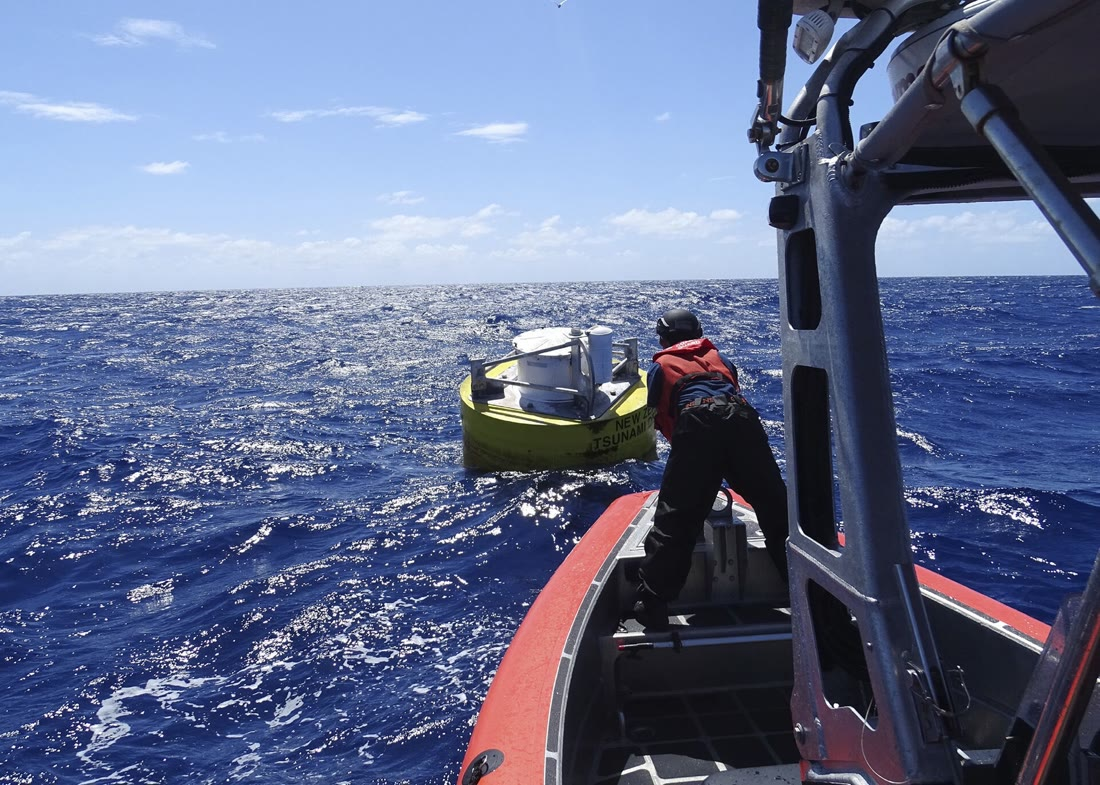
\includegraphics[width=\linewidth]{images/book1/g9-dart-buoy.jpg}
\end{minipage}\hfill
\begin{minipage}[c]{0.56\linewidth}\raggedright
{\small Un membre d'équipage d'un navire des \omterm{def:g1:landscapes-around-us:water}{garde-côtes} des États-Unis
inspecte une bouée d'alerte aux \omterm{def:g7:earthquakes:tsunami}{tsunamis} dans l'\omterm{def:g2:water-on-earth:ocean}{océan} Pacifique, en
novembre 2021. La bouée flotte au-dessus d'un capteur de pression posé sur
le fond de la \omterm{def:g2:water-on-earth:ocean}{mer}, des milliers de mètres plus bas. U.S. Coast Guard
(domaine public, via Wikimedia Commons).}
\end{minipage}
% ledger: commons:dart-buoy
\label{fig:g9:natural-risks:buoy}
\end{omfigure}

\begin{history}[Un réseau de bouées]
En 2001, le premier ensemble de six stations de ce type était achevé,
dans l'\omterm{def:g2:water-on-earth:ocean}{océan} Pacifique. Après le \omterm{def:g7:earthquakes:tsunami}{tsunami} de décembre 2004, qui atteignit
les \omterm{def:g1:landscapes-around-us:water}{côtes} de l'\omterm{def:g2:water-on-earth:ocean}{océan} Indien en l'absence de tout système d'alerte
(\cref{ch:g7:earthquakes}), le réseau s'agrandit~: en mars 2008, il
comptait 39 stations.
\end{history}
% ledger: ndbc:dart

Une alerte ne sauve des vies que si elle atteint des gens qui savent quoi
en faire~: les itinéraires vers les hauteurs sont balisés et connus par
des exercices, le kit d'urgence est prêt, les écoles organisent des
exercices d'évacuation. À Armero, l'aléa était connu et la \omterm{def:g2:drawing-to-map:map}{carte} était
tracée~; l'alerte n'a jamais atteint la ville.
% ledger: ready:kit, usgs:armero

\section{Exercices}

\begin{exercise}[$\star$]\label{exo:g9:natural-risks:1}
Aléa ou \omterm{def:g9:natural-risks:vulnerability}{vulnérabilité}~? (a) Une \omterm{def:g1:landscapes-around-us:water}{rivière} qui déborde presque chaque
printemps. (b) Un village sans système d'alerte. (c) De lourdes maisons de
briques sans ossature. (d) Un fort \omterm{def:g4:volcanoes-earthquakes-first-look:earthquake}{séisme} sur une \omterm{def:g7:earthquakes:fault}{faille} voisine. (e) Une
ville bâtie au débouché d'une \omterm{def:g1:landscapes-around-us:landform}{vallée} où des coulées de boue sont déjà
descendues.
\end{exercise}

\begin{exercise}[$\star$]\label{exo:g9:natural-risks:2}
Vrai ou faux~? Corrige les phrases fausses. (a) Un \omterm{def:g5:natural-hazards:hazard}{aléa naturel} dans un
lieu où personne ne vit est un \omterm{def:g9:natural-risks:risk}{risque} élevé. (b) La \omterm{def:g9:natural-risks:prevention}{prévention} peut
réduire la \omterm{def:g9:natural-risks:vulnerability}{vulnérabilité} d'une ville. (c) Une \omterm{def:g9:natural-risks:hazard-map}{carte des aléas} montre où un
aléa peut frapper. (d) Un bon système d'alerte rend un \omterm{def:g4:volcanoes-earthquakes-first-look:volcano}{volcan} moins
dangereux.
\end{exercise}

\begin{exercise}[$\star$]\label{exo:g9:natural-risks:3}
Pour chaque aléa, dis s'il peut être prévu quelques jours ou quelques
heures à l'avance~: (a) une \omterm{def:g5:natural-hazards:storm}{tempête}~; (b) une \omterm{def:g5:water-shapes-the-land:flood}{crue} après de fortes
\omterm{def:g4:clouds-rain-snow:precipitation}{pluies}~; (c) un \omterm{def:g4:volcanoes-earthquakes-first-look:earthquake}{séisme}~; (d) l'arrivée d'un \omterm{def:g7:earthquakes:tsunami}{tsunami} sur une \omterm{def:g1:landscapes-around-us:water}{côte} éloignée
de son lieu d'origine.
\end{exercise}

\begin{exercise}[$\star$]\label{exo:g9:natural-risks:4}
% ledger: usgs:hvo-toolkit
Utilise le dessin du \omterm{def:g4:volcanoes-earthquakes-first-look:volcano}{volcan} surveillé. Que mesure chaque instrument, et
quel signe avant-coureur d'une \omterm{def:g4:volcanoes-earthquakes-first-look:eruption}{éruption} guette-t-il~? (a) Un \omterm{def:g7:earthquakes:seismometer}{sismomètre}.
(b) Un inclinomètre. (c) Un récepteur GPS. (d) Un analyseur de gaz.
\end{exercise}

\begin{exercise}[$\star\star$]\label{exo:g9:natural-risks:5}
% ledger: usgs:armero
En 1985, les coulées de boue du Nevado del Ruiz atteignirent Armero, à
\qty{45}{km}, environ deux heures après l'\omterm{def:g4:volcanoes-earthquakes-first-look:eruption}{éruption}. (a) Quelle était leur
vitesse moyenne, en kilomètres par heure~? (b) Une personne marche à
environ \qty{4}{km/h}. Quelle distance les habitants auraient-ils pu
parcourir à pied en deux heures~? (c) Pourquoi ne sont-ils pas partis~?
(d) Donne deux choses qui auraient pu les sauver.
\end{exercise}

\begin{exercise}[$\star\star$]\label{exo:g9:natural-risks:6}
% ledger: (invented region: figdata/grade-9/flood_zone.py)
Utilise la \omterm{def:g2:drawing-to-map:map}{carte} des zones inondables des collines de Varden. (a) Quelle
\omterm{def:g5:water-shapes-the-land:flood}{crue} couvre la bande la plus large~? (b) À l'aide du quadrillage de la
\omterm{def:g2:drawing-to-map:map}{carte}, mesure la largeur de chaque zone en travers de la \omterm{def:g1:landscapes-around-us:landform}{vallée} à
\qty{5}{km} est. (c) Une grange est bâtie sur un terrain situé
\qty{6}{m} au-dessus de la \omterm{def:g1:landscapes-around-us:water}{rivière}.
Lesquelles des trois \omterm{def:g5:water-shapes-the-land:flood}{crues} l'atteignent~? (d) Pourquoi la \omterm{def:g5:water-shapes-the-land:flood}{crue} de
\qty{2}{m} au-dessus de la \omterm{def:g1:landscapes-around-us:water}{rivière} est-elle celle qui revient le plus
souvent~?
\end{exercise}

\begin{exercise}[$\star\star$]\label{exo:g9:natural-risks:7}
Place chaque situation sur la grille du \omterm{def:g9:natural-risks:risk}{risque} (aléa faible ou fort,
\omterm{def:g9:natural-risks:vulnerability}{vulnérabilité} faible ou forte) et dis si le \omterm{def:g9:natural-risks:risk}{risque} est faible, moyen ou
élevé. (a) Des bâtiments solides et des exercices dans une ville située
sur une \omterm{def:g7:earthquakes:fault}{faille} active. (b) Un terrain de camping dans la \omterm{def:g5:water-shapes-the-land:flood}{plaine
d'inondation} d'une \omterm{def:g1:landscapes-around-us:water}{rivière} qui déborde rarement. (c) Un village de maisons
fragiles au pied d'un \omterm{def:g4:volcanoes-earthquakes-first-look:volcano}{volcan} actif, sans observatoire. (d) Une ville au
sommet d'une \omterm{def:g1:landscapes-around-us:landform}{colline}, loin de toute \omterm{def:g7:earthquakes:fault}{faille}, \omterm{def:g1:landscapes-around-us:water}{rivière} ou \omterm{def:g4:volcanoes-earthquakes-first-look:volcano}{volcan}.
\end{exercise}

\begin{exercise}[$\star\star$]\label{exo:g9:natural-risks:8}
% ledger: iris:better-wall, explo:base-isolation
Trois écoles sont bâties sur le même terrain. L'école A est une ossature
de poteaux et de poutres avec des murs de briques entre eux~; l'école B a
la même ossature avec des contreventements en diagonale et deux voiles~;
l'école C a l'ossature de B, posée sur des isolateurs. (a) Classe-les de
la plus sûre à la moins sûre en cas de \omterm{def:g4:volcanoes-earthquakes-first-look:earthquake}{séisme}. (b) Explique ce que font
les contreventements. (c) Explique ce que font les isolateurs.
\end{exercise}

\begin{exercise}[$\star\star$]\label{exo:g9:natural-risks:9}
% ledger: fema:flood-zones
Une \omterm{def:g2:drawing-to-map:map}{carte} des zones inondables montre la \omterm{def:g5:water-shapes-the-land:flood}{crue} centennale, qui a une
chance sur 100 d'être atteinte ou dépassée chaque année. (a) Écris cette
chance sous forme de pourcentage. (b) Un voisin dit~: «~La \omterm{def:g5:water-shapes-the-land:flood}{crue}
centennale est venue l'an dernier, donc nous sommes tranquilles pour
99 ans.~» Qu'est-ce qui ne va pas~? (c) En moyenne, combien de \omterm{def:g5:water-shapes-the-land:flood}{crues} de ce
type surviendraient en 300 ans~?
\end{exercise}

\begin{exercise}[$\star\star$]\label{exo:g9:natural-risks:10}
% ledger: ndbc:dart, nws:tsunami-speed
Une station d'alerte aux \omterm{def:g7:earthquakes:tsunami}{tsunamis} mesure la pression sur le fond de la \omterm{def:g2:water-on-earth:ocean}{mer}
toutes les \qty{15}{s}. (a) Combien de mesures fait-elle en une heure~?
(b) En une année de 365 jours~? Écris la réponse en notation
scientifique. (c) Un \omterm{def:g7:earthquakes:tsunami}{tsunami} traverse l'\omterm{def:g2:water-on-earth:ocean}{océan} profond à environ
\qty{800}{km/h}. Combien de temps met-il pour atteindre une \omterm{def:g1:landscapes-around-us:water}{côte} située à
\qty{2400}{km}~? (d) Pourquoi cette durée compte-t-elle~?
\end{exercise}

\begin{exercise}[$\star\star\star$]\label{exo:g9:natural-risks:11}
% ledger: ready:kit
Une famille de quatre personnes prépare un kit d'urgence avec de l'eau pour
3 jours, à raison d'environ \qty{3.8}{L} par personne et par jour, pour
boire et se laver. (a) De combien de litres d'eau a-t-elle besoin~?
(b) Combien de bouteilles de \qty{1.5}{L} cela fait-il~? (c) Nomme quatre
autres objets que contient le kit, et dis à quoi chacun sert. (d) Pourquoi
le kit est-il rangé près de la porte~?
\end{exercise}

\begin{exercise}[$\star\star\star$]\label{exo:g9:natural-risks:12}
% ledger: usgs:armero, usgs:hvo-toolkit
Une ville s'étend au bord d'une \omterm{def:g1:landscapes-around-us:water}{rivière}, au débouché d'une \omterm{def:g1:landscapes-around-us:landform}{vallée} qui
descend d'un \omterm{def:g4:volcanoes-earthquakes-first-look:volcano}{volcan} enneigé. D'anciens \omterm{def:g5:water-shapes-the-land:deposition}{dépôts} de coulées de boue se
trouvent sous ses rues. Le \omterm{def:g4:volcanoes-earthquakes-first-look:volcano}{volcan} a commencé à trembler de petits \omterm{def:g4:volcanoes-earthquakes-first-look:earthquake}{séismes}.
Rédige pour la ville un plan de \omterm{def:g9:natural-risks:prevention}{prévention} en cinq points. Pour chaque
point, dis s'il agit du côté de l'aléa (connaître et surveiller l'aléa) ou
du côté de la \omterm{def:g9:natural-risks:vulnerability}{vulnérabilité}.
\end{exercise}

\section{Problème~: où construire la nouvelle école~?}

\begin{problem}[{Problème du week-end --- une nouvelle école est placée sur
la carte des collines de Varden, à l'écart des crues, des pentes raides et
de la faille~; la réponse finale est le nombre de maisons situées dans la
zone inondable}]
\label{pb:g9:natural-risks:1}
% ledger: (invented region: figdata/grade-9/flood_zone.py: sites A, B, C; 17 of 28 houses in the 5 m zone)
Le village des collines de Varden a besoin d'une nouvelle école, et trois
terrains sont proposés~: A, B et C, sur la \omterm{def:g2:drawing-to-map:map}{carte} ci-dessous. La zone
inondable ombrée sur la \omterm{def:g2:drawing-to-map:map}{carte} est tout le terrain situé à moins de
\qty{5}{m} au-dessus de la \omterm{def:g1:landscapes-around-us:water}{rivière}, qu'une grande \omterm{def:g5:water-shapes-the-land:flood}{crue} recouvrirait. Le
tableau donne, pour chaque terrain, l'\omterm{def:g4:world-physical-map:altitude}{altitude} du sol, le niveau de la
\omterm{def:g1:landscapes-around-us:water}{rivière} à côté, et de combien le sol s'élève sur \qty{200}{m} mesurés à
l'horizontale en travers de la pente.

\begin{center}
{\small
\begin{tabular}{|c|c|c|c|}
\hline
terrain & \omterm{def:g4:world-physical-map:altitude}{altitude} du sol & niveau de la \omterm{def:g1:landscapes-around-us:water}{rivière} à côté & élévation du sol sur \qty{200}{m} \\
\hline
A & \qty{137}{m} & \qty{137}{m} & \qty{1.4}{m} \\
B & \qty{276}{m} & \qty{126}{m} & \qty{83}{m} \\
C & \qty{236}{m} & \qty{143}{m} & \qty{20}{m} \\
\hline
\end{tabular}}
\end{center}

\begin{omfigure}
\begin{tikzpicture}
\begin{axis}[axis equal image, xmin=3.5, xmax=7, ymin=2.7, ymax=5.5, width=11.5cm,
  enlargelimits=false, tick label style={font=\scriptsize}, xlabel={est (km)},
  ylabel={nord (km)}, label style={font=\small}, xtick={3.5,4,...,7}, ytick={3,3.5,...,5.5}]
\addplot[contour] table {figdata/out/grade-9-flood_zone-contours.dat};
\addplot[index contour] table {figdata/out/grade-9-flood_zone-index.dat};
\addplot[fill=blue!25, draw=blue!50, line width=0.3pt] table {figdata/out/grade-9-flood_zone-zone.dat} -- cycle;
\addplot[only marks, mark=none, point meta=explicit symbolic, nodes near coords,
  nodes near coords align={center}, nodes near coords style={font=\tiny, fill=white, inner sep=0.6pt, text=omContour}]
  table[meta=z] {figdata/out/grade-9-flood_zone-index-lab.dat};
\addplot[river] table {figdata/out/grade-9-flood_zone-river.dat};
\addplot[fault] table {figdata/out/shared-region-fault.dat};
\addplot[only marks, mark=square*, mark size=1.5pt, mark options={fill=black}] table {figdata/out/grade-9-flood_zone-houses-in.dat};
\addplot[only marks, mark=square*, mark size=1.5pt, mark options={fill=black}] table {figdata/out/grade-9-flood_zone-houses-out.dat};
\addplot[only marks, mark=*, mark size=2.6pt, mark options={fill=omWarm, draw=black}, point meta=explicit symbolic,
  nodes near coords, nodes near coords align={anchor=south west},
  nodes near coords style={font=\small\bfseries, fill=white, inner sep=1pt, xshift=2.5pt, yshift=2.5pt}]
  table[meta=name] {figdata/out/grade-9-flood_zone-sites.dat};
\node[font=\footnotesize, fill=white, inner sep=1pt, anchor=west] at (axis cs:6.42,5.05) {faille};
\coordinate (na) at (axis cs:3.7,4.75);
\fill[black] (axis cs:5.8,2.85) rectangle (axis cs:5.925,2.9);
\fill[white] (axis cs:5.925,2.85) rectangle (axis cs:6.05,2.9);
\fill[black] (axis cs:6.05,2.85) rectangle (axis cs:6.175,2.9);
\fill[white] (axis cs:6.175,2.85) rectangle (axis cs:6.3,2.9);
\draw[black, line width=0.4pt] (axis cs:5.8,2.85) rectangle (axis cs:6.3,2.9);
\node[font=\footnotesize, above, inner sep=1.5pt, fill=white] at (axis cs:6.05,2.9) {\qty{500}{m}};
\end{axis}
\fill[white, opacity=0.85] ($(na)+(-0.35,-0.1)$) rectangle ($(na)+(0.35,1.45)$);
\pic at (na) {northarrow};
\end{tikzpicture}

{\small Le village, les trois terrains proposés pour l'école et la zone
inondable (ombrée), sur la \omterm{def:g2:drawing-to-map:map}{carte} des collines de Varden (lignes fines de
même \omterm{def:g4:world-physical-map:altitude}{altitude} tous les \qty{10}{m}). Chaque petit carré noir est une
maison. Le trait noir épais est une \omterm{def:g7:earthquakes:fault}{faille}.}
\label{fig:g9:natural-risks:school-map}
\end{omfigure}

\noindent\textbf{Partie I --- La zone inondable.}\par\nopagebreak
\begin{enumerate}[beginpenalty=10000]
  \item À l'aide des niveaux de la \omterm{def:g1:landscapes-around-us:water}{rivière} du tableau, dis dans quel sens
        coule la \omterm{def:g1:landscapes-around-us:water}{rivière}.
  \item Calcule la hauteur de chaque terrain au-dessus de la \omterm{def:g1:landscapes-around-us:water}{rivière} à
        côté.
  \item Lequel des trois terrains se trouve dans la zone inondable~?
  \item Utilise l'\omterm{def:g2:drawing-to-map:scale}{échelle} graphique pour mesurer la largeur de la zone
        inondable, en travers de la \omterm{def:g1:landscapes-around-us:landform}{vallée}, au terrain~A.
\end{enumerate}

\noindent\textbf{Partie II --- Les pentes et la faille.}\par\nopagebreak
\begin{enumerate}[resume, beginpenalty=10000]
  \item Une pente en pourcentage est l'élévation du sol pour
        \qty{100}{m} mesurés à l'horizontale. Calcule la pente de chaque
        terrain.
  \item Quel terrain serait exposé à un \omterm{def:g5:natural-hazards:landslide}{glissement de terrain}~? Explique.
  \item Utilise l'\omterm{def:g2:drawing-to-map:scale}{échelle} graphique pour estimer la distance de chaque
        terrain à la \omterm{def:g7:earthquakes:fault}{faille}.
  \item Suppose que la \omterm{def:g7:earthquakes:fault}{faille} puisse encore jouer. Pourquoi le terrain
        situé juste au-dessus est-il un mauvais emplacement pour une
        école~?
\end{enumerate}

\noindent\textbf{Partie III --- Choisir.}\par\nopagebreak
\begin{enumerate}[resume, beginpenalty=10000]
  \item Trace un tableau avec une ligne par terrain et trois colonnes~:
        dans la zone inondable~? pente raide~? sur la \omterm{def:g7:earthquakes:fault}{faille}~? Remplis-le
        avec oui ou non.
  \item Quel terrain choisirais-tu~? Justifie ton choix à l'aide du
        tableau.
  \item Le terrain choisi se trouve encore dans une région où le sol peut
        trembler. Donne deux façons de construire l'école, et une habitude
        de ses élèves, qui réduisent sa \omterm{def:g9:natural-risks:vulnerability}{vulnérabilité}.
  \item L'école servira aussi d'abri pendant les \omterm{def:g5:water-shapes-the-land:flood}{crues}. Compte les maisons
        du village situées dans la zone inondable. Quelle fraction de
        l'ensemble des maisons cela représente-t-il~?
\end{enumerate}
\end{problem}
